\chapter{How Species Change}\label{ch:g9:how-species-change}

The evidence hall established the fact; this chapter builds
the engine. Its parts are all in your hands already:
\omterm{prop:g9:genes-and-dna:explains}{mutation} writing new spellings
(\cref{prop:g9:genes-and-dna:explains}), the shuffle dealing
unique decks (\cref{prop:g9:unique-individuals:theorem}),
the \omterm{def:g6:exploring-our-environment:components}{environment}'s checks collecting most of every
generation's surplus
(\cref{prop:g8:reproduction-and-environment:limits}).
Assembled, they run themselves --- that self-running is
\omterm{prop:g9:how-species-change:selection}{natural selection}, and it is the most consequential simple
idea in \omterm{def:g1:living-or-not:living}{biology}.

\section{The engine, assembled}

\begin{proposition}[Natural selection]\label{prop:g9:how-species-change:selection}
Three facts, none deniable, and their consequence:
\begin{enumerate}
  \item \emph{variety}: a \omterm{def:g8:reproduction-and-environment:population}{population}'s individuals differ
        in inherited \omterm{def:g9:heredity-and-traits:traits}{traits}
        (\cref{prop:g9:unique-individuals:reserve} banked
        it);
  \item \emph{over-production and checks}: far more young
        are produced than the \omterm{def:g6:exploring-our-environment:components}{environment} lets survive ---
        the checks collect the surplus
        (\cref{ex:g8:reproduction-and-environment:twosprings});
  \item \emph{unequal collection}: the checks do not
        collect at random --- individuals whose inherited
        \omterm{def:g9:heredity-and-traits:traits}{traits} suit the current \omterm{def:g6:exploring-our-environment:conditions}{conditions} escape them a
        little more often, and so leave more offspring,
        \emph{who inherit those \omterm{def:g9:heredity-and-traits:traits}{traits}}.
\end{enumerate}
Consequence: generation after generation, the suited
\omterm{def:g9:genes-and-dna:gene}{alleles}' share of the \omterm{def:g8:reproduction-and-environment:population}{population} grows. That drift of a
\omterm{def:g8:reproduction-and-environment:population}{population}'s inherited makeup, driven by nothing but
variety meeting checks, is \emph{natural
selection}\index{natural selection} --- and enough time
makes it \emph{evolution}\index{evolution}.
\end{proposition}
\admitted

\begin{example}[The moths, mechanized]\label{ex:g9:how-species-change:moths}
\Cref{ex:g9:evidence-of-evolution:live}'s peppered moths,
part by part. Variety: pale and dark inherited forms.
Checks: \omterm{prop:g3:sorting-living-things:groups}{birds} hunt moths by sight against bark.
Unequal collection: on soot-blackened trunks the pale form
is the visible one --- eaten more, so the dark \omterm{def:g9:genes-and-dna:gene}{allele}'s
share climbs toward the observed dark woods; the air
clears, the bark pales, and the same engine runs in
reverse. No moth changed; the \emph{\omterm{def:g8:reproduction-and-environment:population}{population}'s} makeup
did --- selection edits the deck's frequencies, not the
individuals.
\end{example}

\begin{omfigure}
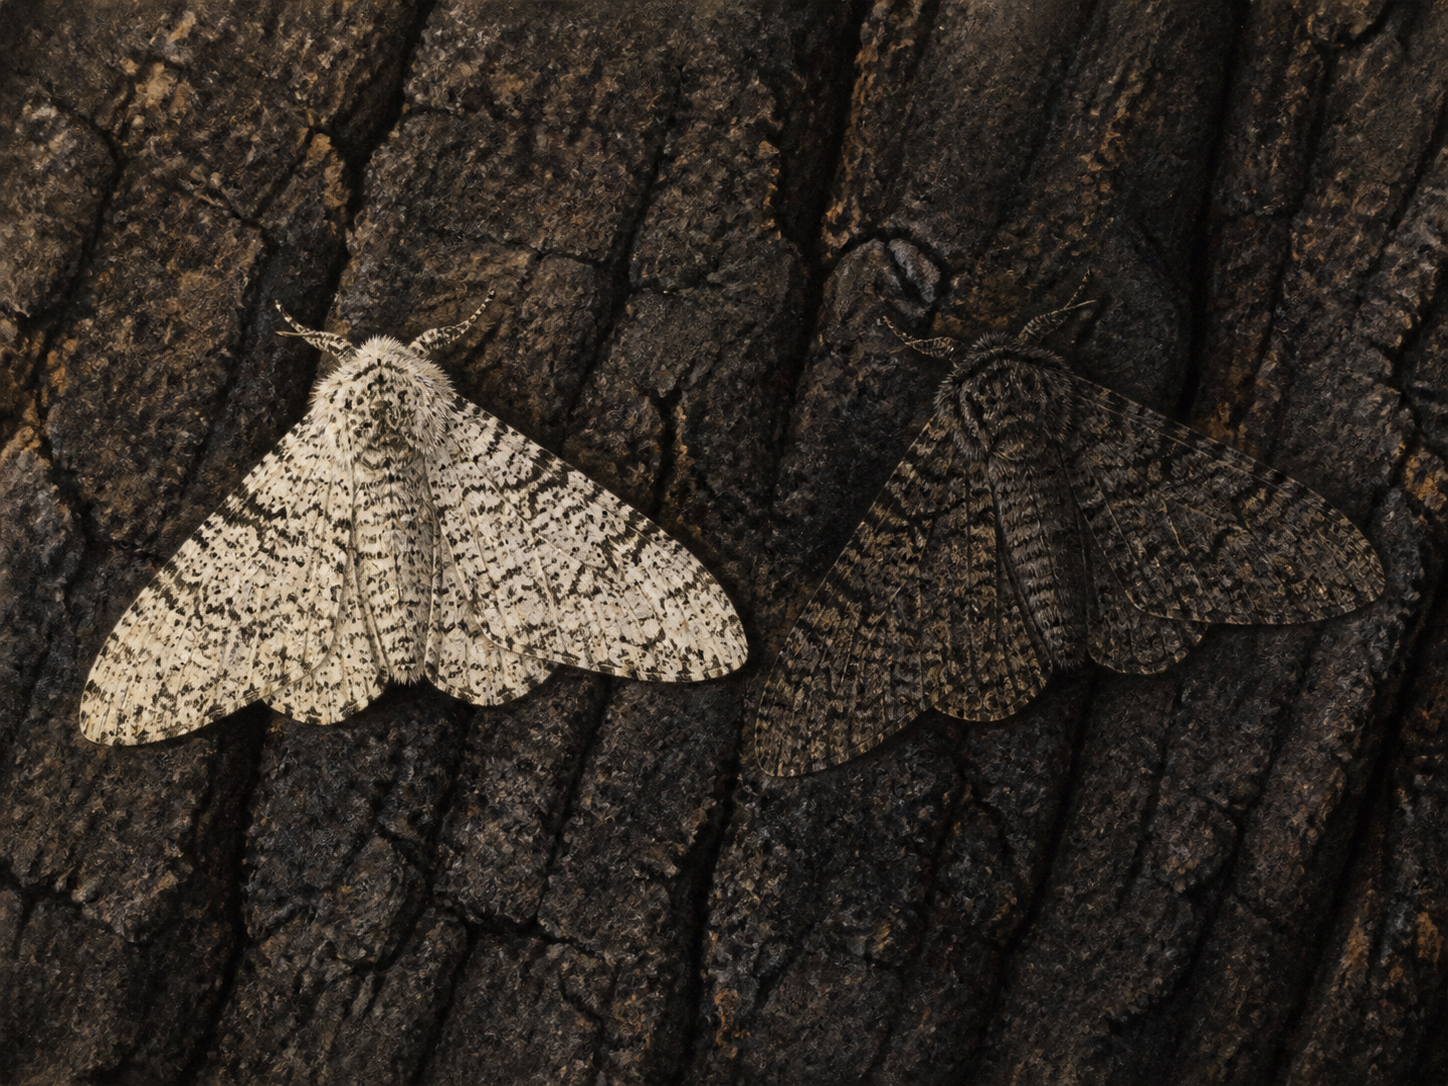
\includegraphics[width=0.56\linewidth]{images/book1/ai/g9-moths-bark.png}

{\small The check at work: on soot-stained bark, the pale
form is the visible one --- and the visible one is the eaten
one.}
\end{omfigure}

\begin{remark}[What selection is not]\label{rem:g9:how-species-change:not}
Three standing confusions, retired:
\begin{itemize}
  \item \emph{no intention}: \omterm{def:g6:exploring-our-environment:conditions}{conditions} select the way
        dampness ``selected'' woodlice
        (\cref{ex:g6:exploring-our-environment:chooser})
        --- by consequences, not choices; nothing plans;
  \item \emph{no perfection}: selection only compares the
        variants \emph{present} --- it finds the better
        available, not the best imaginable (the shared
        \omterm{def:g1:my-body:parts}{limb} plan's awkward re-jobbing,
        \cref{exo:g9:evidence-of-evolution:7}, is its
        signature);
  \item \emph{no inheritance of effort}: the blacksmith's
        \omterm{def:g1:my-body:parts}{arm} dies with the blacksmith
        (\cref{prop:g9:heredity-and-traits:sorting});
        selection works only on what \omterm{def:g8:sexual-reproduction:gametes}{gametes} carry.
        Giraffes did not stretch their necks long ---
        longer-necked variants out-fed and out-bred the
        shorter.
\end{itemize}
\end{remark}

\section{The engine observed and exploited}

\begin{example}[Selection in the hospital]\label{ex:g9:how-species-change:resistance}
The medical case, mechanized for
\cref{ch:g9:microbes-and-infection}'s use: a microbe
\omterm{def:g8:reproduction-and-environment:population}{population} holds rare resistant mutants
(\omterm{prop:g9:genes-and-dna:explains}{mutation}'s trickle); an antibiotic is the check; it
collects the susceptible and spares the resistant, who
inherit the ward. Days, not millennia --- generations
turn in hours, and selection's speed scales with them.
Every rule about finishing antibiotic courses and not
scattering antibiotics into farming is engine management:
weaken the check raggedly, and you breed what you meant
to kill.
\end{example}

\begin{example}[Selection with a human hand on the check]\label{ex:g9:how-species-change:artificial}
\Cref{pb:g8:sexual-reproduction:1}'s breeder ran the same
engine with herself as the check --- keeping the crisp and
resistant, culling the rest. Every dog breed, every \omterm{def:g6:producing-our-food:farming}{crop}
variety, every dairy line is accumulated
\emph{artificial selection}: proof of the engine's power
on a human timescale, wolf to lapdog inside some thousands
of generations. Darwin --- the naturalist who assembled
this chapter's argument --- opened his great book with
exactly that comparison.
\end{example}

\begin{omfigure}
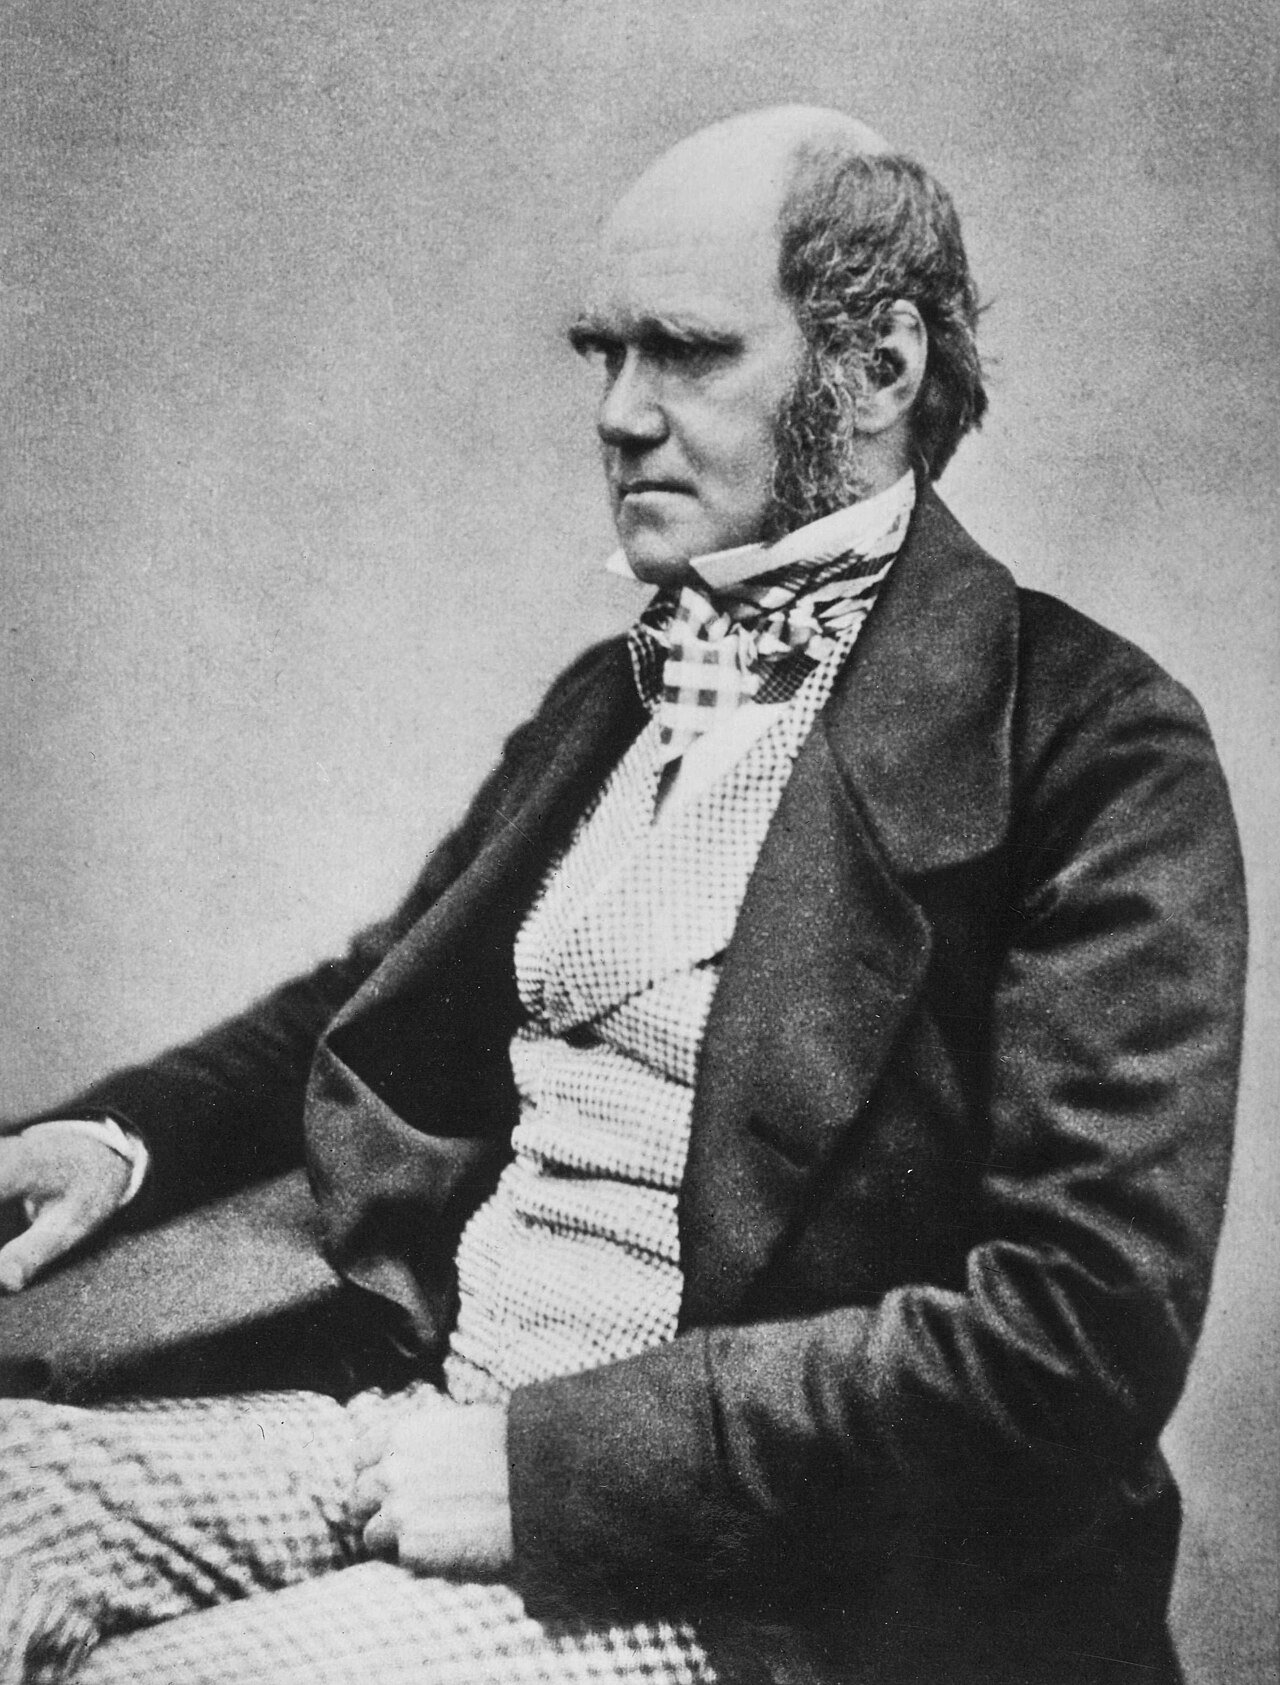
\includegraphics[width=0.42\linewidth]{images/book1/darwin.jpg}

{\small Charles Darwin, photographed around 1854, in the
years he was assembling this chapter's argument.}
\end{omfigure}

\begin{proposition}[From change to new species]\label{prop:g9:how-species-change:speciation}
Selection explains a \omterm{def:g8:reproduction-and-environment:population}{population} changing; one more
ingredient explains \omterm{def:g8:reproduction-and-environment:population}{populations} \emph{splitting}.
Separate two \omterm{def:g8:reproduction-and-environment:population}{populations} of one \omterm{def:g5:biodiversity:species}{species} --- a sea rises,
a range divides, an island receives castaways
(\cref{exo:g6:how-plants-spread:11}) --- and each runs
the engine under its own \omterm{def:g6:exploring-our-environment:conditions}{conditions}, accumulating its own
\omterm{def:g9:genes-and-dna:gene}{alleles}. Given enough divergence, the two no longer
interbreed where they meet: by
\cref{def:g5:biodiversity:species}'s own definition, two
\omterm{def:g5:biodiversity:species}{species} stand where one stood. The tree's forks
(\cref{def:g6:classification-kinship:tree}) are exactly
such splits, deep time's worth of them.
\end{proposition}
\admitted

\begin{method}[Running the engine on any case]\label{met:g9:how-species-change:run}
For any claimed example of \omterm{prop:g9:how-species-change:selection}{evolution}:
\begin{enumerate}
  \item name the \emph{variety} and check it is inherited
        (\cref{met:g9:heredity-and-traits:audit});
  \item name the \emph{check}, and how it collects
        unequally across that variety;
  \item follow the \emph{bookkeeping}: whose \omterm{def:g9:genes-and-dna:gene}{alleles} gain
        share in the next generation?
  \item for a split, add the \emph{separation} and the
        diverging \omterm{def:g6:exploring-our-environment:conditions}{conditions};
  \item timescale check: generations, not years, are the
        engine's ticks.
\end{enumerate}
\end{method}

\section{Exercises}

\begin{exercise}[$\star$]\label{exo:g9:how-species-change:1}
State \omterm{prop:g9:how-species-change:selection}{natural selection}'s three facts and their
consequence.
\end{exercise}

\begin{exercise}[$\star$]\label{exo:g9:how-species-change:2}
In the moth case, name variety, check, and the unequal
collection --- in both directions.
\end{exercise}

\begin{exercise}[$\star$]\label{exo:g9:how-species-change:3}
What changes under selection --- the individuals, or the
\omterm{def:g8:reproduction-and-environment:population}{population}? Explain.
\end{exercise}

\begin{exercise}[$\star$]\label{exo:g9:how-species-change:4}
Correct, mechanism in hand: ``giraffes stretched their
necks and passed the stretch on.''
\end{exercise}

\begin{exercise}[$\star$]\label{exo:g9:how-species-change:5}
Why does antibiotic resistance evolve in days where moths
took decades?
\end{exercise}

\begin{exercise}[$\star$]\label{exo:g9:how-species-change:6}
What did the apple breeder and the moth's \omterm{prop:g3:sorting-living-things:groups}{birds} have in
common, and what differed?
\end{exercise}

\begin{exercise}[$\star\star$]\label{exo:g9:how-species-change:7}
Why can selection not produce ``the best imaginable''
organism? Which of its three facts limits it?
\end{exercise}

\begin{exercise}[$\star\star$]\label{exo:g9:how-species-change:8}
Run \cref{met:g9:how-species-change:run} on the finches'
drought (\cref{ex:g9:evidence-of-evolution:live}): \omterm{prop:g3:flowers-fruits-seeds:transform}{seeds}
harden, big beaks crack what small ones cannot.
\end{exercise}

\begin{exercise}[$\star\star$]\label{exo:g9:how-species-change:9}
Assemble speciation for the island castaways of
\cref{exo:g6:how-plants-spread:11}: separation,
divergence, and the test that would declare two \omterm{def:g5:biodiversity:species}{species}.
\end{exercise}

\begin{exercise}[$\star\star$]\label{exo:g9:how-species-change:10}
Explain, engine in hand, why unfinished antibiotic
courses and farm-scattered antibiotics both breed
resistance.
\end{exercise}

\begin{exercise}[$\star\star$]\label{exo:g9:how-species-change:11}
``Selection is the checks of
\cref{ch:g8:reproduction-and-environment}, falling on the
variety of \cref{ch:g9:unique-individuals}.'' Justify the
sentence as the book's own summary.
\end{exercise}

\begin{exercise}[$\star\star\star$]\label{exo:g9:how-species-change:12}
Why does the engine \emph{need} \omterm{def:g4:animal-reproduction:sexual}{sexual reproduction}'s
shuffle and \omterm{prop:g9:genes-and-dna:explains}{mutation}'s trickle --- what happens to
selection in a \omterm{def:g8:reproduction-and-environment:population}{population} of perfect clones
(\cref{exo:g9:unique-individuals:8}) once \omterm{def:g6:exploring-our-environment:conditions}{conditions}
turn?
\end{exercise}

\section{Problem: The Island Notebooks}

\begin{problem}[{Weekend problem --- two centuries on a
volcanic archipelago}]\label{pb:g9:how-species-change:1}
A (composite, historically inspired) archipelago:
volcanic islands, never joined to the mainland, hosting
finch-like \omterm{prop:g3:sorting-living-things:groups}{birds} whose beak forms differ island to
island --- and differ from their one evident mainland
kin. Naturalists' notebooks span two centuries.

\medskip\noindent\textbf{Part I --- The pattern.}
\begin{enumerate}
  \item The islands hold only \omterm{def:g5:biodiversity:species}{species} that could cross
        the sea --- \omterm{prop:g3:sorting-living-things:groups}{birds}, \omterm{prop:g3:flowers-fruits-seeds:transform}{drift-seeds}, one bat, no
        native land \omterm{prop:g3:sorting-living-things:groups}{mammals} or frogs. Which chapter
        predicted the passenger list
        (\cref{exo:g6:how-plants-spread:11})?
  \item All the archipelago's finches resemble the one
        mainland \omterm{def:g5:biodiversity:species}{species} more than any other bird on
        Earth. What does \omterm{prop:g6:classification-kinship:kinship}{kinship} reasoning
        (\cref{prop:g6:classification-kinship:kinship})
        conclude about their origin?
  \item Beaks differ by island's diet: seed-crackers on
        \omterm{def:g2:from-seed-to-plant:seed}{seed} islands, probers on cactus islands. Read
        the match with
        \cref{prop:g4:adapted-to-their-world:answers} ---
        then say what this chapter adds that the
        \omterm{def:g4:adapted-to-their-world:adaptation}{adaptation} chapter could not.
  \item Why are volcanic, never-joined islands the
        engine's showcase? Name the speciation
        ingredient they supply wholesale.
\end{enumerate}

\medskip\noindent\textbf{Part II --- The engine's
notebook years.}
\begin{enumerate}[resume]
  \item A drought year: soft \omterm{prop:g3:flowers-fruits-seeds:transform}{seeds} fail, hard \omterm{prop:g3:flowers-fruits-seeds:transform}{seeds}
        remain; the ringers' calipers show next year's
        hatchlings averaging deeper beaks. Run the
        engine's bookkeeping through that sentence.
  \item Wet years follow, soft \omterm{prop:g3:flowers-fruits-seeds:transform}{seeds} return, and the
        average drifts back. What does the reversal
        prove about selection's ``direction''?
  \item One island's finches, transplanted by storm to
        another, breed poorly with the residents. Which
        proposition is being watched mid-run?
  \item A creationist-era notebook objects: ``no one has
        seen one \omterm{def:g5:biodiversity:species}{species} become another.'' Answer with
        timescale and the convergent-witness method
        (\cref{met:g9:evidence-of-evolution:weigh}).
\end{enumerate}

\medskip\noindent\textbf{Part III --- The synthesis
lecture.}
\begin{enumerate}[resume]
  \item Deliver the archipelago's story in the engine's
        five steps
        (\cref{met:g9:how-species-change:run}), castaway
        arrival to island \omterm{def:g5:biodiversity:species}{species}.
  \item Explain why every island's finch is ``the better
        available, not the best imaginable'' --- what
        could each island's deck offer selection?
  \item Connect the archipelago to the hospital ward of
        \cref{ex:g9:how-species-change:resistance}: same
        engine, different tick rate --- state what sets
        the rate.
  \item Close the lecture with Darwin's comparison made
        explicit: what the pigeon-fancier's hand and the
        drought's hard \omterm{prop:g3:flowers-fruits-seeds:transform}{seeds} have in common.
\end{enumerate}
\end{problem}
